\documentclass{article}

\usepackage{booktabs}
\usepackage{tabularx}
\usepackage{graphicx}
\usepackage{float}

\usepackage{xcolor}
\usepackage{ulem}

\title{Development Plan\\\prognam}

\author{Smita Singh, Abeer Alyasiri, Niyatha Rangarajan,\\ Moksha Srinivasan, Nicholas Lobo, Longwei Ye}
\date{September 25, 2022}

%%% Comments

\usepackage{color}

\newif\ifcomments\commentstrue %displays comments
%\newif\ifcomments\commentsfalse %so that comments do not display

\ifcomments
\newcommand{\authornote}[3]{\textcolor{#1}{[#3 ---#2]}}
\newcommand{\todo}[1]{\textcolor{red}{[TODO: #1]}}
\else
\newcommand{\authornote}[3]{}
\newcommand{\todo}[1]{}
\fi

\newcommand{\wss}[1]{\authornote{blue}{SS}{#1}} 
\newcommand{\plt}[1]{\authornote{magenta}{TPLT}{#1}} %For explanation of the template
\newcommand{\an}[1]{\authornote{cyan}{Author}{#1}}

%%% Common Parts

\newcommand{\progname}{ProgName} % PUT YOUR PROGRAM NAME HERE
\newcommand{\authname}{Team \#, Team Name
\\ Student 1 name and macid
\\ Student 2 name and macid
\\ Student 3 name and macid
\\ Student 4 name and macid} % AUTHOR NAMES                  

\usepackage{hyperref}
    \hypersetup{colorlinks=true, linkcolor=blue, citecolor=blue, filecolor=blue,
                urlcolor=blue, unicode=false}
    \urlstyle{same}
                                


\begin{document}


\maketitle

\begin{table}[hp]
\caption{Revision History} \label{TblRevisionHistory}
\begin{tabularx}{\textwidth}{llX}
\toprule
\textbf{Date} & \textbf{Developer(s)} & \textbf{Change}\\
\midrule
Sept. 21, 2022 & Abeer & Introduction, Team Members Roles, Proof of Concept Demonstration, Project Scheduling, Coding Standard \\\\
Sept. 21, 2022 & Smita & Worked on Team Meeting Plan, Team Communication Plan, Workflow Plan, Technology, Coding Standard\\\\
Sept. 25, 2022 & Niyatha & Basic edits for grammatical issues. Suggested better 
 development tools and risk mitigation.\\\\
\textcolor{blue}{Nov. 23, 2022} & \textcolor{blue}{Abeer} & \textcolor{blue}{update POC plan} \\\\
%... & ... & ...\\
\bottomrule
\end{tabularx}
\end{table}

\newpage

\maketitle

This document will explore the development plan of Capstone project in terms of team logistics, project design, testing plan, and project execution %A

\section{Team Meeting Plan}
The plan is to hold meetings every Monday evening from 6:30 to 7:30pm. Meetings will be conducted through Microsoft Teams or when necessary will be held in-person at McMaster's Hatch building. A meeting agenda will be established before each meeting in order to keep the meeting succinct and on track. Agendas will be recorded using OneNote on the Microsoft Team's channel. The meetings will be used for division of labour, and completing deliverables. %S
Other meetings will be held to conduct group work sessions to complete assigned tasks. These meetings will be less formal and will be scheduled based on the project scheduling.

\section{Team Communication Plan}
The primary form of communication will be through Microsoft teams, but a secondary form will be discord for urgent communication. Scheduling meetings and distributing tasks will be communicated through a shared Microsoft Teams channel. %S

\section{Team Member Roles} 
All team members are expected to be responsible for completing technical software component to the project. The default roles assigned for the moment is to divide general topics across the project for members to have more knowledge than others. A deliverable leader will be assigned during the first meeting of each deliverable and the role will be rotated across the team. Deliverable leader is a way for the team to keep track of tasks and ensure the last version is complete for grading. 
\begin{table}[H]
    \centering
    \begin{tabular}{|c|c|p{60mm}|}
         \hline
         Name & Primary Role & Description\\
         \hline
         Moksha Srinivasan & Team Leader & Primary Ticket Creator, Developer\\
         \hline
         Abeer Alyasiri & Scribe & Liason between TA and supervisor, Developer\\
         \hline
         Nicholas Lobo & Git Expert & Managing and resolving git conflicts, Developer \\
         \hline
         Niyatha Rangarajan & Documentation Expert & Responsible for managing documentation, Developer \\
         \hline
         Longwei Ye & Technology Expert & Responsible for gaining knowledge on new technologies, Developer  \\
         \hline
         Smita Singh & LaTeX Expert & Responsible for resolving latex errors, Developer \\
         \hline
    \end{tabular}
    \caption{Team Roles}
    \label{tab:team_roles}
\end{table}
%A

\section{Workflow Plan} %S

The team will be using a main branch to store stable code. Every feature, bug fix or code refactor will require a new branch to be made from main and then a pull request would need to be created. Each pull request must be reviewed and approved by two other members of the team in order for it to be merged into the main branch. This will ensure a decrease in error prone code being added to the main branch. The pull request will be merged as a squash commit.

Issues will be discussed and created by all of the group members and will be stored in the GitHub issue tracker. Issues will be classified by three classes: feature, bug, and refactor. Each member will be assigned issues every week to work on when the implementation process has started. The team will establish team specific milestones, in order to keep track with deadlines and deliverables. 

\section{Proof of Concept Demonstration Plan} %A

\subsection{Most Significant Risk}
The project will include three main risks that the team must address for a successful demonstration. The first one is scalability of the software to meet the project scope. This includes module designs related to performance and maintainability. The project is tackling multiple aspects of the ARC GIS system so it is important to design modules following the separation of concerns principles to ensure modularity in the design. Building a reliable design plan before implementation eliminates the risk. The second risk is the project's functional capabilities within the specified deadlines since the project will be based on the ARC GIS system which include various components for GPS tracking. Hence, the team must prioritize the designing and implementing modules of core functionalities before expanding. This ensures completion of a system with fundamental features. The third risk is re-implementation of existing modules and tools of the system. The team must deliver a full Python3 re-implementation the system with accessible tools for technical users to follow and use. 

\subsection{Will a part of the implementation be difficult?}
The team is not anticipating many problems with implementation except ensuring that only accessible libraries and tools are used to build the system. It may require more research and time to use the new technology with the team's existing set of skills. 

\subsection{Will testing be difficult?}
Automated integration testing for multiple modules will be difficult because it requires enormous amount of work to gather proper data on how the modules will be used together. Therefore, automating such cases might not be feasible for the project.

\subsection{Is a required library difficult to install?}
No, because any required libraries will be available in the project's git repository.

\subsection{Will portability be a concern?}
No, since the project will have all the files available on the git repository as it is open source. Also, the potential users for the software are assumed to have prior knowledge to download the repository and run a starting Python3 module to use the system. Therefore, any technical user with Python pre-installed will be able to use the system.

\subsection{Hardware Concerns}
Not applicable for the project because no hardware is involved. 

\subsection{Proof of Concept Plan}
The proof of concept demonstration will be providing \sout{a summary of the design architecture of the project and showing the fundamental modules in the form of a} use case scenario \textcolor{blue}{run through of the input type, input processing, and expected output format}. The scenario\sout{s} must provide successful system functionalities to ensure proper design decisions, mitigation method for design risks, and technical feasibility to complete the project scope. The demonstration will showcase \sout{all} the \textcolor{blue}{rudimentary} functional features of the system \textcolor{blue}{required} for re-implementation \textcolor{blue}{of the toolbox} \sout{on a rudimentary level} to prove that the system is suitable for scaling \sout{and follows a modular design principle}. \sout{Also, demonstrating 80-90\%} \textcolor{blue}{The demonstration will cover 30-40\%} of the project's main goals. \textcolor{blue}{It} will establish that the team is \sout{successful} \textcolor{blue}{on track to implement the open source toolbox functionality by end of April.} \sout{at completing the project end to the end.}

%What will you demonstrate during your proof of concept demonstration to convince yourself that you will be able to overcome this risk?

%describe what you will demonstrate to show the risks can be overcome
%if the risks prove to be real we can redefine your project
%what technologies we plan to use to show the demo
%design and architecture to be used 
%methods of overcoming risks 


\section{Technology}%S

\subsection{Programming Language}
The team will be using Python3 as the main programming language. Python is a great language for handling large data sets and for computing and performing statistical analysis. \sout{The team may also use some R for certain features if/when necessary.}

\subsection{Development Tools}
 The team will also be using VSCode along with RStudio as an IDE. The linting tool that will be used is pylint in order to keep our code consistent and clean. The team will be likely using the R5py python library for routing different types of transportation networks. As well as GeoPandas which makes geo-spatial data easier to work with in Python. The data will be stored and fetched from MongoDB. GitHub is where the repository will be stored and issues will be created and tracked.
 
\subsection{Documentation}
Doxygen will be used to create documentation for the code. Quarto files will be also be used in parallel to document the code in a more thorough manner. Quarto files will include markdown as well as code in order to create well documented code that is executable.

\subsection{Testing Frameworks}
The unit testing framework that will be used is pytest. Pytest also has various plugins such as pytest-regressions which will be used to regression test our code.
 
\subsection{Continuous Integration}
Continuous Integration will be integrated through GitHub Actions, which will build the code and run the tests on virtual machines hosted by GitHub. CI tests are needed to pass during the pull request stage for the code to be merged in.


\section{Coding Standard}
The project coding standard will follow the Pylint rules. This is because all team members will be using VS Code for Python and will enable the standard linting tool. This will ensure consistent, clean and readable code because Pylint is able to catch a number of bugs and disable unwanted warnings. %A
PEP 8 – Style Guide for Python Code is another tool be used to ensure standard coding conventions. %S

\section{Project Scheduling} %A
The project schedule will be showcased using a Microsoft Planner that will be accessible in the Microsoft Teams channel so all the team members have access to view and update their progress directly on there. The team decided not to follow the recommended approach with Gantt Chart for project scheduling because it is not user friendly to make changes on and during team meetings. The team will be updating the planner to assign what parts each member will be responsible for and a leader to keep track of the milestone progress. Also, each team member will spend approximately 10 hours a week to complete deliverable sections and individual capstone course work. All tasks completed will be communicated on the planner with the description section.
\begin{figure}[h]
\caption{Current state of the planner while working on Problem Statement and Development Plan}
\centering
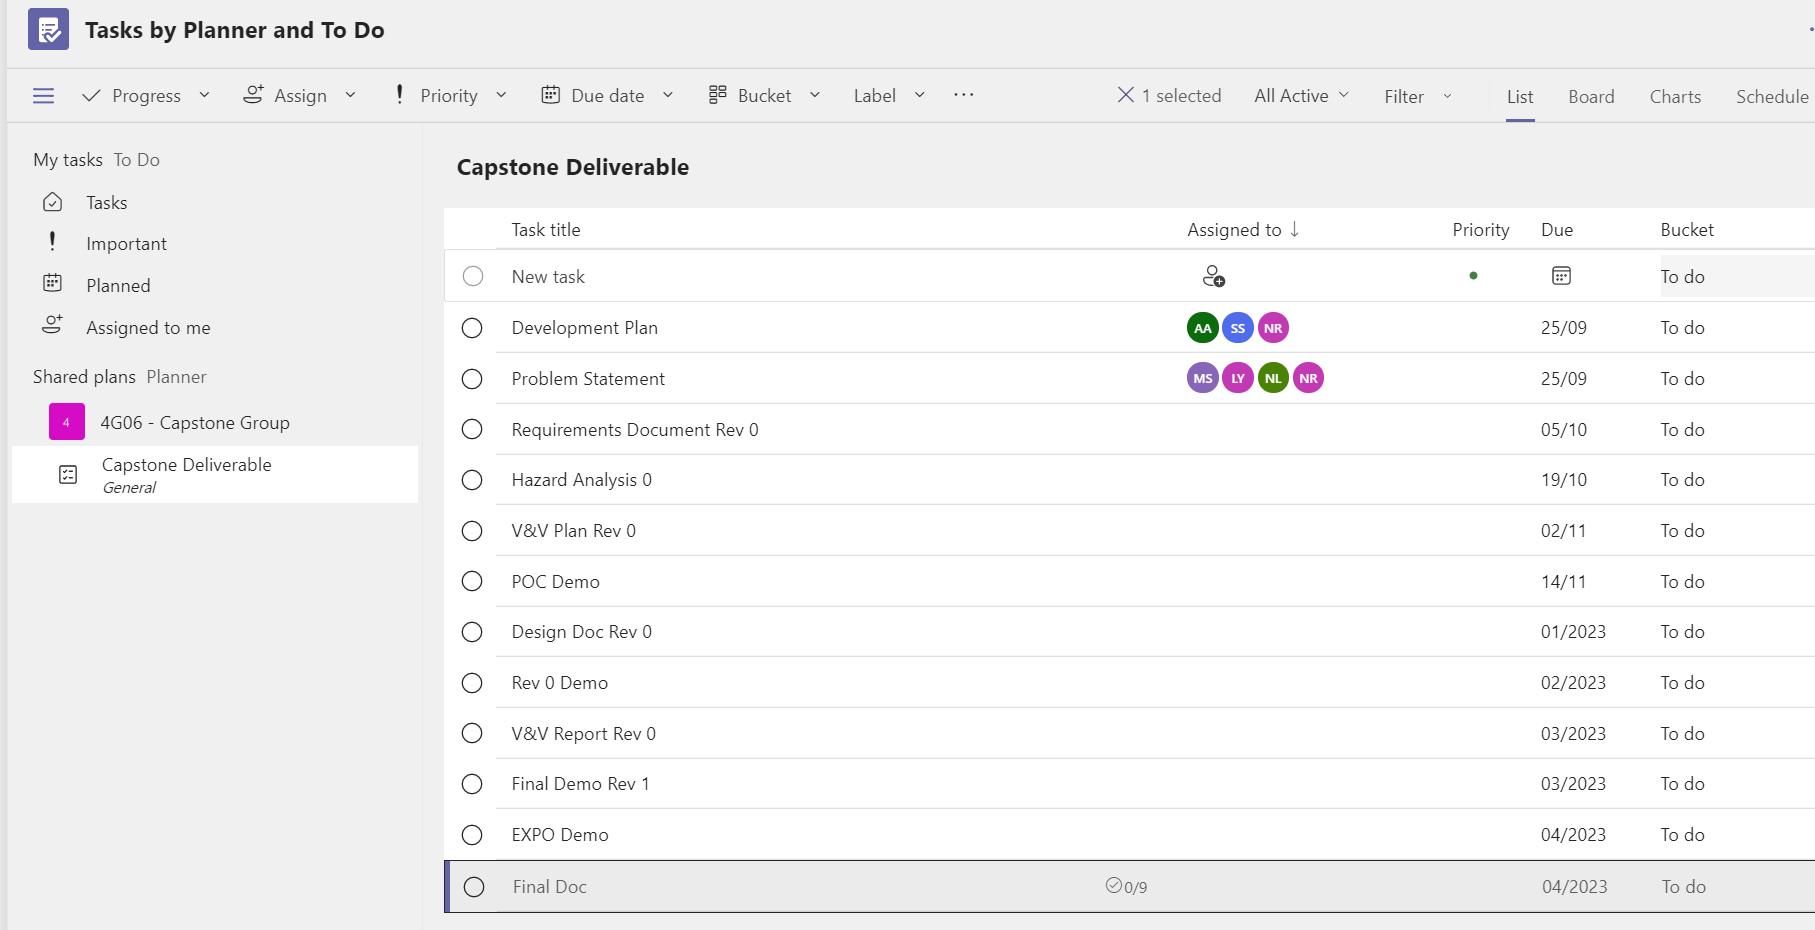
\includegraphics[width=\textwidth]{REV0/DevelopmentPlan/SProject schedule.png}
\end{figure}


\end{document}
